\chapter{Graphical Models}
%
%
%
\section{Modeling}
Modeling our knowledge formally is essential to acquire a model language that can be used with standardized algorithms for learning and inference. %
In this lecture, we use graphical models, i.e. graphs, as a model language. %
A vertex in the graph is an event (or random variable) that may occur and an edge between vertices symbolizes a dependence. %
%
%
%
\subsection{Graph Definitions}
\begin{minipage}[t]{1\textwidth}
	\begin{minipage}[t]{.48\textwidth}
		\begin{figure}[H]
			\centering\resizebox{1\textwidth}{!}{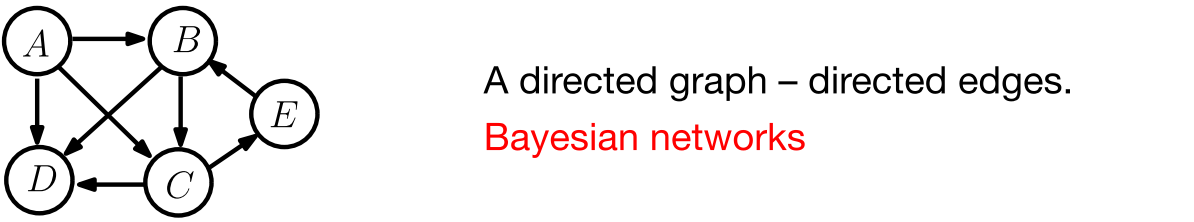
\includegraphics[scale=1]{\mlmedia/03_bayesian_network.png}}
		\end{figure}
	\end{minipage}
	\hfill
	\begin{minipage}[t]{.48\textwidth}
		\begin{figure}[H]
			\centering\resizebox{1\textwidth}{!}{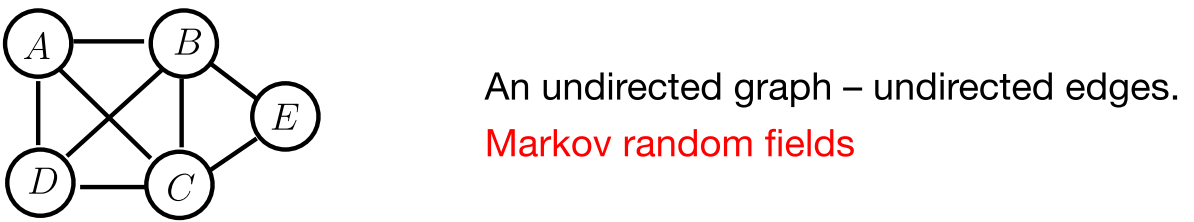
\includegraphics[scale=1]{\mlmedia/03_markov_random_field.png}}
		\end{figure}
	\end{minipage}
\end{minipage}
\vspace*{5pt}
% % %
\begin{itemize}
%
	% Vertex
	\item\itab{Vertex}
	\htab{A vertex is a single node, e.g. \ensuremath{A}, within a graph.}
%
	% Edge
	\item\itab{Edge}
	\htab{An edge is a tuple of vertices, e.g. \ensuremath{(A_1,A_2)}.}
%
	% Directed graph
	\item\itab{Directed Graph}
	\htab{A directed graph has directed edges.}
%
	% Path
	\item\itab{Path}
	\htab{A path from vertex \ensuremath{A} to vertex \ensuremath{B} is denoted as \ensuremath{A\rightarrow B}, a sequence of vertices \ensuremath{A,\;C,\;E,\;B}.}
%
	% Ancestor
	\item\itab{Ancestor}
	\htab{All vertices \ensuremath{A} are ancestors of \ensuremath{B} iff \ensuremath{A\rightarrow B} and \ensuremath{B\not\rightarrow A} in directed graphs.}
%
	% Descendant
	\item\itab{Descendant}
	\htab{All vertices \ensuremath{B} are descendants of \ensuremath{A} iff \ensuremath{A\rightarrow B} and \ensuremath{B\not\rightarrow A} in directed graphs.}
%
	% Undirected graph
	\item\itab{Undirected Graph}
	\htab{An undirected graph has undirected edges.}
%
	% Neighbor
	\item\itab{Neighbor}
	\htab{All neighbors of a vertex \ensuremath{A} in an undirected graph share an edge with \ensuremath{A}.}
%
	% Clique
	\item\itab{Clique}
	\htab{A clique within an undirected graph is a subset of vertices that are fully connected.}
%
	% Maximal clique
	\item\itab{Maximal clique}
	\htab{A clique is called maximal clique if it is not extended by adding another vertex.}
%
	% Directed Acyclic Graph
	\item\itab{Directed Acyclic Graph (DAG)}
	\htab{A graph with directed edges where every vertex will be visited once along a path.}
\end{itemize}
% % %
\begin{figure}[H]
\centering\resizebox{.65\textwidth}{!}{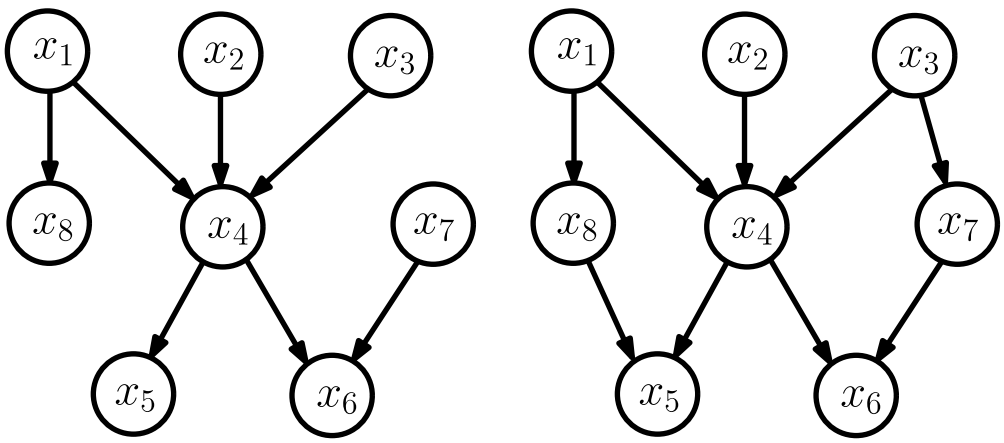
\includegraphics{\mlmedia/03_DAG.png}}
\label{fig:DAG}
\caption{Two exemplary directed acyclic graphs (DAGs) which are sufficient to understand before introducing further terminology.}
\end{figure}
% % %
\begin{itemize}
%
	% Parents
	\item\itab{Parents}
	\htab{The parent of e.g. vertex \ensuremath{x_4} are \ensuremath{pa(x_4) = \{x_1,x_2,x_3\}}.}
%
	% Children
	\item\itab{Children}
	\htab{The children of e.g. vertex \ensuremath{x_4} are \ensuremath{ch(x_4) = \{x_5,x_6\}}.}
%
	% Family
	\item\itab{Family}
	\htab{The family of e.g. vertex \ensuremath{x_4} is \ensuremath{\{x_4\}\cup pa(x_4)\cup ch(x_4)}.}
%
	% Markov Blanket
	\item\itab{Markov Blanket}
	\htab{The Markov blanket of a vertex is given by its parents, children and its children parents.}
%
	% Connected graph
	\item\itab{Connected graph}
	\htab{A graph is connected if there is a path between any two vertices, otherwise there are connected components.}
%
	% Connected components
	\item\itab{Connected components}
	\htab{If a graph is no connected graph, we speak of connected components.}
\end{itemize}
% % %
\begin{figure}[H]
\centering\resizebox{.65\textwidth}{!}{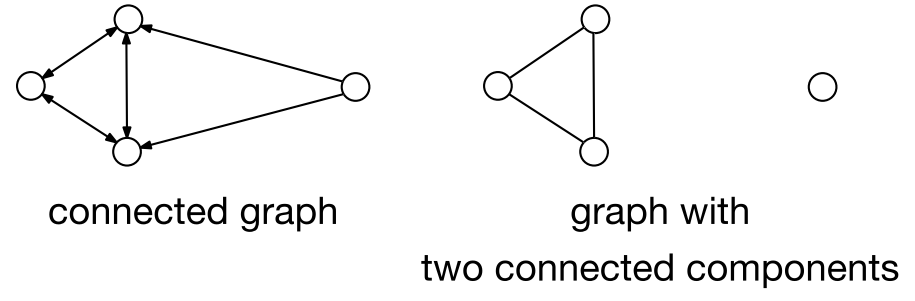
\includegraphics[scale=1]{\mlmedia/03_connected_graph_and_components.png}}
\label{fig:graph_connections}
\end{figure}
% % %
\begin{itemize}
%
	% Singly-connected graph
	\item\itab{Singly-connected graph}
	\htab{There is at most one path between any vertices \ensuremath{A} and \ensuremath{B} in a singly-connected graph.}
%
	% Multiply-connected graph
	\item\itab{Multiply-connected graph}
	\htab{Whenever a graph is no singly-connected graph, it is a multiply-connected graph.}
\end{itemize}
% % %
\begin{figure}[H]
\centering\resizebox{.65\textwidth}{!}{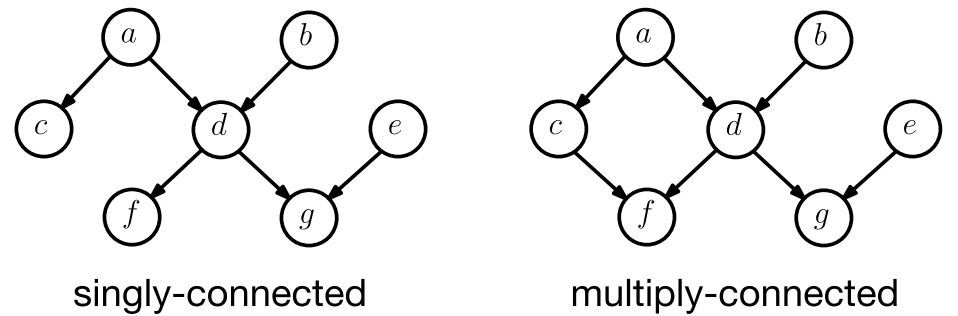
\includegraphics[scale=1]{\mlmedia/03_singly-connected_multiply-connected.png}}
\label{fig:singly_multiply_connected}
\end{figure}
% % %
%
%
%
\subsection{Bayesian Networks / Belief Networks}
\begin{figure}[H]
\centering\resizebox{.7\textwidth}{!}{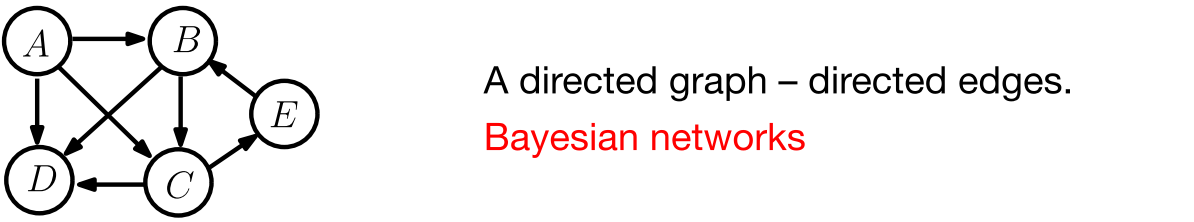
\includegraphics[scale=1]{\mlmedia/03_bayesian_network.png}}
\end{figure}
% % %
A Bayesian network or belief network is a distribution of the form %
\begin{equation}
p( x_1 , \ldots , x_D ) = \prod_{i=1}^{D} p\left( x_i \middle| pa( x_i ) \right).
\label{eq:bayesian_network}
\end{equation}
% % %
A Bayesian network can have different factorizations, e.g. a Bayesian network of the form \ensuremath{p( x_1 , x_2 , x_3 , x_4 )} has two factorizations: %
\begin{figure}[H]
\centering\resizebox{.65\textwidth}{!}{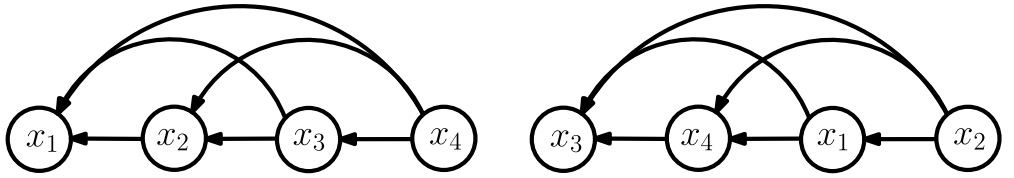
\includegraphics[scale=1]{\mlmedia/03_BN_factorization.png}}
\label{fig:BN_factorizations}
\end{figure}
% % %
\begin{equation*}
p(x_1|x_2,x_3,x_4) p(x_2|x_3,x_4) p(x_3|x_4) p(x_4) = p(x_1,x_2,x_3,x_4) = p(x_3|x_1,x_2,x_4) p(x_4|x_1,x_2) p(x_1|x_2) p(x_2)
\end{equation*}
% % %
Any distribution can be written as a factorization - a cascade form of a belief network - that becomes increasingly important when making independence assumptions. %
The structure of DAGs not only prevents cyclic reasoning but also corresponds to a set of conditional independence assumptions. %
% % %
\subsubsection{Conditional independence}%
Can we read off the conditional independence statements of a given graph? Is there an automatic algorithm? %
\begin{minipage}[t]{1\textwidth}
	\begin{minipage}[t]{.18\textwidth}
		\begin{figure}[H]
			\resizebox{1\textwidth}{!}{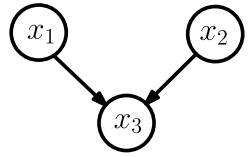
\includegraphics[scale=1]{\mlmedia/03_BN_collider.png}}
		\end{figure}
	\end{minipage}
	\hfill%
	\begin{minipage}[t]{.78\textwidth}
		To answer the questions; yes, we are able to read off the conditional independence in any belief network formally. %
		For this purpose, we define a vertex as a \emph{collider} if there are at least two directed edges pointing to that vertex. %
		We can see such a collider \ensuremath{x_3} depicted in the Figure to the left. %
		Furthermore, we introduce \emph{D-seperation} (or \emph{dependence seperation}) as a tool to check for conditional and unconditional independence. %
		In contrast to D-seperation, we introduce \emph{D-connectedness} (or \emph{dependence connectedness}) to check for conditional and unconditional dependence. %
	\end{minipage}
\end{minipage}
% % %
\subsubsection{D-seperation}%
\fbox{%
\parbox{.98\textwidth}{%
	Lets check for conditional indpendence \ensuremath{\mathcal{X} \CI \mathcal{Y} \mid \mathcal{Z}} in any belief network. %
	For every \ensuremath{x\in\mathcal{X}} and \ensuremath{y\in\mathcal{Y}} check every path \ensuremath{\mathcal{U}} between \ensuremath{x} and \ensuremath{y}. %
	A path is characterized to be \emph{blocked} if there exists a vertex \ensuremath{u\in\mathcal{U}} such that either %
	\begin{enumerate}
		\item \ensuremath{u} \textbf{is a} collider and neither \ensuremath{u} nor any descendant is in \ensuremath{\mathcal{Z}} or
		\item \ensuremath{u} \textbf{is no} collider in \ensuremath{\mathcal{U}} and \ensuremath{u\in\mathcal{Z}}. %
	\end{enumerate}
	If we can show that all such paths \ensuremath{\mathcal{U}} are blocked then \ensuremath{\mathcal{X}} and \ensuremath{\mathcal{Y}} are \emph{d-seperated} by \ensuremath{\mathcal{Z}}. %
	Consequently, the conditional indpendence \ensuremath{\mathcal{X} \CI \mathcal{Y} \mid \mathcal{Z}} does hold. %
}}%
% % %
\subsubsection{D-connectedness}%
\fbox{%
\parbox{.98\textwidth}{%
	The opposite case of D-seperation is D-connectedness. %
	Hence, we check for conditional dependence statement \ensuremath{{\mathcal{X} \CD \mathcal{Y} \mid \mathcal{Z}}} in any belief network. %
	We say that \ensuremath{\mathcal{X}} and \ensuremath{\mathcal{Y}} are \emph{d-connected} by \ensuremath{\mathcal{Z}} iff they are not d-seperated by \ensuremath{\mathcal{Z}}. %
	Consequently, the conditional dependence \ensuremath{\mathcal{X} \CD \mathcal{Y} \mid \mathcal{Z}} does hold if \ensuremath{\mathcal{X}} and \ensuremath{\mathcal{Y}} are d-connected. %
}}%
% % %
\subsubsection{Markov equivalence}
\fbox{%
\parbox{.98\textwidth}{%
	Two graphs are Markov equivalent if they represent the same set of conditional independence statements. %
	More precisely this means that the two graphs have the same \emph{skeleton} and the same set of \emph{immoralities}. %
	\\[.2cm]%
	\begin{minipage}[t]{.95\textwidth}
		\begin{minipage}[t]{.78\textwidth}
			\begin{itemize}
				\item\itab{Skeleton}\tab{resulting graph after removing all arrows of all edges}
				\item\itab{Immorality}\tab{the parents of a child have no connection, i.e. ``are unmarried''\\(cf. the graph at the right as an example)}
			\end{itemize}
		\end{minipage}
		\hfill%
		\begin{minipage}[t]{.18\textwidth}
			\vspace*{-.5cm}
			\begin{figure}[H]
				\resizebox{1\textwidth}{!}{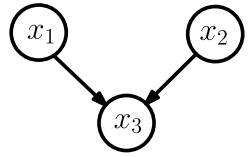
\includegraphics[scale=1]{\mlmedia/03_BN_collider.png}}
			\end{figure}
		\end{minipage}
	\end{minipage}
	\\%
	Note that the Markov equivalence holds for both, directed and undirected graphs. %
}}%
%
%
%
\subsection{Markov Random Fields}
\begin{figure}[H]
\centering\resizebox{.7\textwidth}{!}{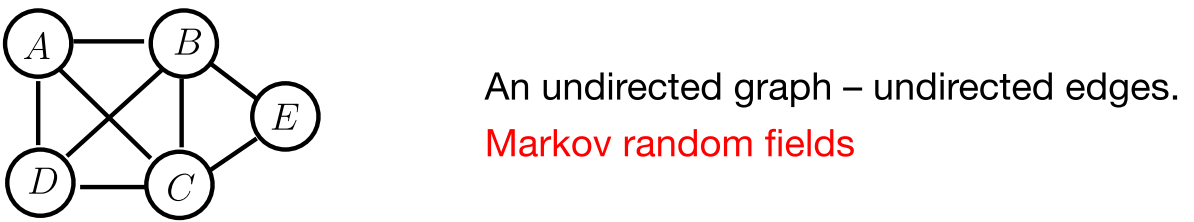
\includegraphics[scale=1]{\mlmedia/03_markov_random_field.png}}
\end{figure}
So far, we considered factorizations of probability distributions with normalized factors so that the product will again result in the probability distribution. %
Alternatively we could factorize with so called \emph{potential function} \ensuremath{\phi(x)} as follows %
\begin{equation}
p(a,b,c) = \frac{1}{Z} \phi(a,b) \phi(b,c)
\label{eq:alternative_factorization}
\end{equation}%
with an explicit normalization constant called \emph{partition function} \ensuremath{Z} defined as %
\begin{equation}
Z = \sum_{a}\sum_{b}\sum_{c} \phi(a,b) \phi(b,c).
\label{eq:partition_function}
\end{equation}%
A \emph{potential function} is a non-negative function \ensuremath{\phi(x)} of the input \ensuremath{x} and a \emph{joint potential function} is a non-negative function \ensuremath{\phi(x_1,\ldots,x_D)} of a set of variables. %
\\[.3cm]%
\subsubsection{Definition of a Markov Random Field}
\fbox{%
\parbox{.98\textwidth}{%
	A \emph{Markov Random Field} (\emph{MRF}) (or \emph{Markov Network}) is defined as a product of potentials for a set of variables \ensuremath{\mathcal{X} = \{x_1,\ldots,x_D\}} over the maximal cliques \ensuremath{\mathcal{X}_c} of a graph and is denoted as in Equation~(\ref{eq:MRF}). %
	\begin{equation}
		p(x_1,\ldots,x_D) = \frac{1}{Z} \prod_{c=1}^{C} \phi_c(\mathcal{X}_c)
		\label{eq:MRF}
	\end{equation}
	There is the special case of the \emph{pairwise MRF} where the clique sizes \ensuremath{\{\forall c\in C : |\mathcal{X}_c|\} = \{2\}}. %
	However, in the case that all potentials are strictly positive, we are talking of a \emph{Gibbs distribution}. %
}}%
\clearpage
% % %
\subsubsection{Properties of a Markov Random Field}
\fbox{%
\parbox{.98\textwidth}{%
	\begin{minipage}[t]{.95\textwidth}
		\begin{minipage}[t]{.78\textwidth}
			We subsequently consider the Markov network depicted to the right to explain general properties of Markov networks. %
			The Markov network has the factorization %
			\begin{equation}
				p(a,b,c) = \frac{1}{Z} \phi_{ac}(a,c) \phi_{bc}(b,c)
				\label{eq:MRF_properties}
			\end{equation}
		\end{minipage}
		\hfill%
		\begin{minipage}[t]{.18\textwidth}
			\vspace*{-.5cm}
			\begin{figure}[H]
				\resizebox{1\textwidth}{!}{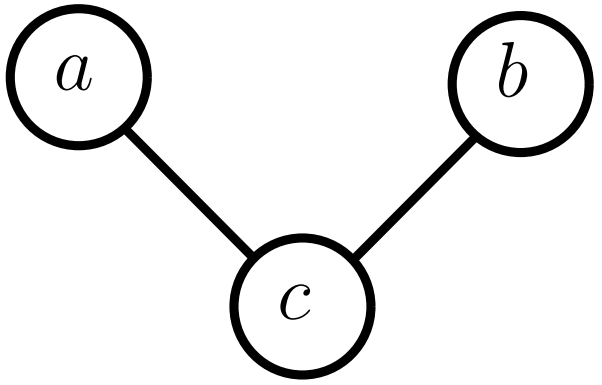
\includegraphics[scale=1]{\mlmedia/03_Markov_Network.png}}
			\end{figure}
		\end{minipage}
	\end{minipage}
	\begin{itemize}[leftmargin=55pt]
		\item[\textbf{Property 1.}] Marginalization of vertex \ensuremath{c} in Equation~(\ref{eq:MRF_properties}) makes the vertices \ensuremath{a} and \ensuremath{b} ``graphically'' dependent, i.e. a new edge between \ensuremath{a} and \ensuremath{b} arises. %
%
		\item[\textbf{Property 2.}] Conditioning Equation~(\ref{eq:MRF_properties}) on the vertex \ensuremath{c} makes the vertices \ensuremath{a} and \ensuremath{b} inpendent, i.e. \ensuremath{{p(a,b\mid c)} = {p(a\mid c) p(b\mid c)}}. %
%
		\item[\textbf{Property 3.}] The \emph{local Markov property} states that each vertex has a condition on its neighbors and is independent on all other vertices. %
		This property is formalized in Equation~(\ref{eq:loca_markov_property}) %
		\begin{equation}
			p(x\mid \mathcal{X}\textbackslash\{x\}) = p(x\mid \NE(x))
			\label{eq:loca_markov_property}
		\end{equation}
%
		\item[\textbf{Property 4.}] The \emph{global Markov property} states that for disjoint sets of variables \ensuremath{(\mathcal{X},\mathcal{Y},\mathcal{Z})} %
		\begin{equation}
			\mathcal{X} \CI \mathcal{Y} \mid \mathcal{Z}
		\end{equation}%
		holds where \ensuremath{\mathcal{Z}} seperates \ensuremath{\mathcal{X}} from \ensuremath{\mathcal{Y}}. %
	\end{itemize}
}}%
\\[.3cm]%
% % %
The Hammersley-Clifford Theorem states sufficient conditions to specify independence statements in an undirected graph. %
Thus it gives necessary and sufficient conditions under which a positive probability distribution can be represented as a Markov network. %
\\[.3cm]%
\subsubsection{Hammersley-Clifford Theorem}
\fbox{%
\parbox{.98\textwidth}{%
The Hammersley-Clifford Theorem states that a non-negative probability distribution satisfies one of the upper Markov properties with respect to an undirected graph iff it is a Gibbs random field. %
In this case, the density can be factorized over the cliques of the graph (or subgraph).
}}%
\\[.3cm]%
% % %
So how do we check for conditional independence of undirected graphs? %
We discussed this issue already for belief networks but this can barely be a general approach because of the directed edges. %
Hence we work out a general algorithm to check for conditional independence here for directed and undirected graphs. %
We define \ensuremath{\mathcal{D} = \{\mathcal{X} \cup \mathcal{Y} \cup \mathcal{Z}\}} for the subsequent algorithm. %
\\[.1cm]%
\begin{enumerate}
	\item\itab{\emph{Ancestral Graph}}%
	\tab{We can build up an ancestral graph by removing all vertices \ensuremath{A} with all their edges from the graph for which hold that \ensuremath{A\not\in\mathcal{D}} and \ensuremath{A} is no ancestor of any vertices \ensuremath{B\in\mathcal{D}}.}%
%
	\item\itab{\emph{Moralization}}%
	\tab{Moralize the ancestral graph from the previous step by connecting parents with their common child and striping all the directions from the edges.}%
%
	\item\itab{\emph{Seperation}}%
	\tab{Remove edges that link to neighbors in \ensuremath{\mathcal{Z}} and if there is no path between a vertex in \ensuremath{\mathcal{X}} to a vertex in \ensuremath{\mathcal{Y}} we know that the conditional independence \ensuremath{\mathcal{X} \CI \mathcal{Y} \mid \mathcal{Z}} holds.}
\end{enumerate}
Finally, we introduce the relationship between directed and undirected graphical models. %
Both, directed and undirected graphical models, imply set of conditional indpendences. %
% % %
\\[.3cm]
\begin{minipage}[t]{1\textwidth}
	\begin{minipage}[t]{.48\textwidth}
		\centerline{\Large{}D map (dependency map)}
		\vspace*{5pt}
		\begin{itemize}
			\item Every conditional independence statement, satisfied by the distribution, is reflected in the graph
			\item A completely disconnected graph contains all possible independence statements for its variables, i.e. is a trivial \emph{D map} for any distribution
		\end{itemize}
		~\\%
	\end{minipage}
	\hfill
	\vrule
	\hfill
	\begin{minipage}[t]{.48\textwidth}
		\centerline{\Large{}I map (independence map)}
		\vspace*{5pt}
		\begin{itemize}
			\item Every conditional independence statement, reflected in the graph, is satisfied by the distribution
			\item A fully connected graph contains all possible dependence statements for its variables, i.e. is a trivial \emph{I map} for any distribution
		\end{itemize}
		~\\%
	\end{minipage}
\end{minipage}
~\\[.3cm]
We can now derive \emph{perfect map}s in terms of \emph{D map}s and \emph{I map}s. %
A perfect map is, both, a D map and an I map of a distribution. %
More precisely, every conditional independence statement satisfied by a distribution is reflected in the corresponding graph and vice versa. %
%
%
%
\subsection{Factor Graphs}
\begin{minipage}[t]{.96\textwidth}
	\begin{minipage}[t]{.68\textwidth}
		We already learned about different graph structures. %
		They all had in common that they implicitly encode the factorization, no matter if directed or undirected. %
		This leads to multiple factorizations of e.g. an undirected Markov random field as can be seen in the Figure to the right. %
		However, the factorization of a \emph{factor graph} (FG) is not specified by the graph itself, thus we use an (formally) explicit factorization. %
		The factorizations are presented with an extra node or vertex; the symbol is a black square. %
	\end{minipage}
	\hfill
	\begin{minipage}[t]{.28\textwidth}
		\begin{figure}[H]
			\centering\resizebox{1\textwidth}{!}{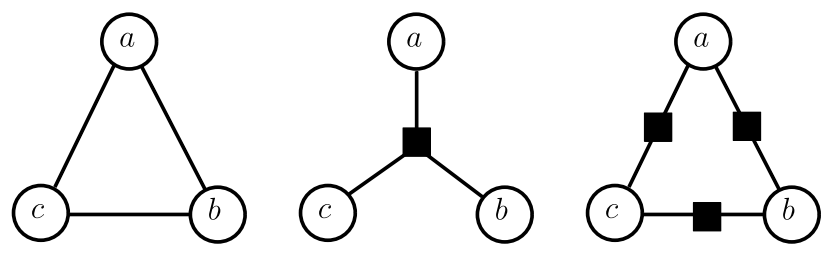
\includegraphics[scale=1]{\mlmedia/03_factor_graph_MRF.png}}
		\end{figure}
	\end{minipage}
\end{minipage}
\\[.1cm]%
% % %
\subsubsection{Factor Graphs}
\fbox{%
\parbox{.98\textwidth}{%
	\begin{minipage}[t]{.96\textwidth}
		\begin{minipage}[t]{.68\textwidth}
			Given a function of the form %
			\begin{equation*}
			f(x_1,\ldots,x_D) = \prod_i \psi_i(\mathcal{X}_i),
			\end{equation*}
			the factor graph has as abovementioned an extra node or vertex for each factor \ensuremath{\psi_i(\mathcal{X}_i)} and a variable node or vertex for each variable \ensuremath{x_j}. %
			Each factor is connected to the variables of which it is a function. %
			When we use factor graphs to represent a distribution of the form %
		\end{minipage}
		\hfill
		\begin{minipage}[t]{.28\textwidth}
			%\hspace*{-5cm}
			\begin{figure}[H]
				\centering\resizebox{1\textwidth}{!}{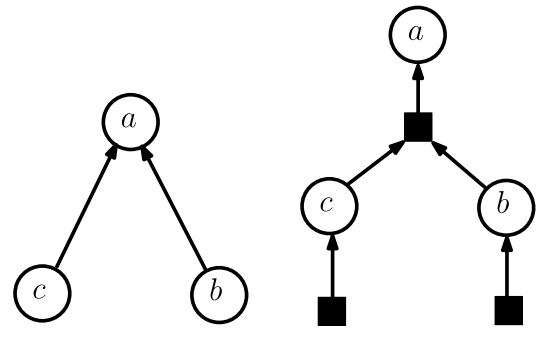
\includegraphics[scale=1]{\mlmedia/03_factor_graph_BN.png}}
			\end{figure}
		\end{minipage}
	\end{minipage}
	\begin{equation}
		p(x_1,\ldots,x_D) = \frac{1}{Z} \prod_i \psi_i(\mathcal{X}_i)
		\label{eq:factor_graph}
	\end{equation}
	we tend to assume a normalization constant \ensuremath{Z}. %
	The Figure on the right shows such an exemplary factor graph of a belief network \ensuremath{c \rightarrow a \leftarrow b}. %
}}%
\\[.3cm]%
\subsubsection{Bipartite graph}
\fbox{%
\parbox{.98\textwidth}{%
	A bipartite graph has vertices that can be divided into two disjoint sets \ensuremath{U} and \ensuremath{V} of vertices such that every edge connects a vertex in the subset \ensuremath{U} with a vertex of subset \ensuremath{V}. %
}}%
%
%
%
\section{Inference in graphical models}
We exploited different structures to model probability distributions \ensuremath{p(x_1,\ldots,x_D)}. %
However, how do we infer, i.e. computing functions like mean, marginal, and conditionals, in these structures? %
%
%
%
%\subsection{Marginalization}\label{sec:marginalization_graphical_models}
\\[.1cm]%
We start with marginalization / \emph{variable elimination}. %
Assume a Markov chain \ensuremath{A \leftarrow B \leftarrow C \leftarrow D} with \ensuremath{A,B,C,D\in\{0,1\}}. %
The distribution of this Markov chain is given by \ensuremath{p(A,B,C,D) = p(A\mid B) p(B\mid C) p(C\mid D) p(D)}. %
We seek the solution \ensuremath{p(A)} which is given by %
\begin{equation}
\begin{aligned}
p(A) &= \sum_B \sum_C \sum_D p(A,B,C,D)\\
	 &= \sum_B \sum_C \sum_D p(A\mid B) p(B\mid C) p(C\mid D) p(D)
\end{aligned}
\end{equation}
which is also quite heavy in computation (\ensuremath{8 = 2^3} computations). %
Here, we can use the linearity property of the summation and reorder the term as follows %
\begin{equation}
p(A) = \sum_B \sum_C p(A\mid B) p(B\mid C) \sum_D p(C\mid D) p(D)
\end{equation}
with subsequent functional substitution %
\begin{equation}
\begin{aligned}
p(A) &= \sum_B \sum_C p(A\mid B) p(B\mid C) \underbrace{\sum_D p(C\mid D) p(D)}_{\gamma_D(C)} \\
p(A) &= \sum_B p(A\mid B) \underbrace{\sum_C p(B\mid C) \gamma_D(C)}_{\gamma_C(B)} \\
p(A) &= \sum_B p(A\mid B) \gamma_C(B).
\end{aligned}
\end{equation}
Now we only need \ensuremath{2+2+2 = 6} computations and for a Markov chain of arbitrary length the computation time scales linearly. %
%
%
%
%\subsection{Conditional marginals}
\\[.1cm]%
Furthermore, we will use the marginalization from above and the fact that \ensuremath{p(D\mid A) \propto p(A,D)} to find the conditional marginals of the Markov chain \ensuremath{A \leftarrow B \leftarrow C \leftarrow D} with \ensuremath{A,B,C,D\in\{0,1\}}. %
The resulting term \ensuremath{\gamma_C(D)} (cf. lecture slides) is no probability distribution and hence need to be normlized with the sum over all possible outcome \ensuremath{\left(\sum_D\gamma_C(D)\right)^{-1}}.
We will end up with a representation depicted in Figure~(\ref{fig:factor_graph_MC}). %
We will interpret \ensuremath{\gamma_C(D)} as \emph{message} because it is not a probability distribution. %
\begin{figure}[H]
\centering\resizebox{.5\textwidth}{!}{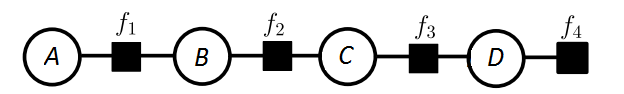
\includegraphics[scale=1]{\mlmedia/03_factor_graph_MC.png}}
\caption{Factor graph representation of a Markov chain \ensuremath{A\leftarrow B\leftarrow C\leftarrow D}.}
\label{fig:factor_graph_MC}
\end{figure}
If now also take the factors into account, we end up with the following: %
\begin{itemize}
	\item We aim to compute the conditional marginal \ensuremath{p(D\mid A)} as follows. %
\end{itemize}
\begin{equation}
\begin{aligned}
p(D\mid A) &\propto p(A,D) = p(A,B,C,D)\\
&= \sum_B \sum_C f_1(A,B)\cdot f_2(B,C)\cdot f_3(C,D)\cdot f_4(D)\\
&= \sum_C \underbrace{\sum_B f_1(A,B)\cdot f_2(B,C)}_{\mu_{A\rightarrow C}(C)}\cdot f_3(C,D)\cdot f_4(D)\\
&= \underbrace{\sum_C \mu_{A\rightarrow C}(C)\cdot f_3(C,D)}_{\mu_{A\rightarrow D}(D)}\cdot f_4(D)\\
&= \mu_{A\rightarrow D}(D)\cdot f_4(D)\\
\end{aligned}
\end{equation}
The advantage here, we only need to compute messages once and can reuse them at any time (as long as the outcome within these messages does not change). %
A \emph{message} \ensuremath{\mu_{m\rightarrow n}(n)} can be understood as an information carrier from \ensuremath{m} to \ensuremath{n} where we still have to choose \ensuremath{n} (and hence it is still parameterized). %
But how do we compute messages efficiently? %
%
%
%
\subsection{Sum-Product algorithm / Belief propagation}\label{sec:belief_propagation}
We will derive the \emph{sum-product algorithm} considering a singly-connected graph. %
We are able to compute any desired marginals with this algorithm. %
\begin{enumerate}
	\item \itab{Initalization}
	\htab{
		Message from extremal (simplical) node factors are initialized to the factor
		\begin{equation}
		\mu_{f\rightarrow x}(x) = f(x)
		\end{equation}
		Message from extremal (simplical) variable nodes are set to unity
		\begin{equation}
		\mu_{f\rightarrow x}(x) = 1
		\end{equation}
	}
	\item \itab{Variable-to-Factor message}
	\htab{
		\begin{equation}
			\mu_{x\rightarrow f}(x) = \prod_{g\in\{ \NE(x)\textbackslash \{f\} \}} \mu_{g\rightarrow x}(x)
			\label{eq:var2fac}
		\end{equation}
	}
	\item \itab{Factor-to-Variable message}
	\htab{
		\begin{equation}
			\mu_{f\rightarrow x}(x) =
			\sum_{\mathcal{X}_f \textbackslash \{x\}} \phi_f(\mathcal{X}_f) 
			\prod_{y\in\{ \NE(f)\textbackslash \{x\} \}} \mu_{y\rightarrow f}(y)
			\label{eq:fac2var}
		\end{equation}
	}
\end{enumerate}
\subsubsection{Message ordering}%
Note that there are two orderings defined on messages. %
This fact is important because a message always dependes on its previous message. %
However, extremal nodes and factors do not depend on other messages. %
To compute all messages in a graph, we compute from \emph{leaf-to-root} (pick root node, compute messages pointing towards root) and \emph{root-to-leaf} (compute messages pointing away from root). %
\\[.3cm]%
%
%
%
\subsubsection{Log-Messages}%
Using logarithmic messages is quite reasonable in large graph because the messages may become very small. %
The belief propagation algorithm from Section~(\ref{sec:belief_propagation}) changes accordingly in Equations~(\ref{eq:var2fac})~and~(\ref{eq:fac2var}) as follows %
\begin{itemize}
	\item\itab{Variable to log Factor message}
	\htab{
		\begin{equation}
		\lambda_{x\rightarrow f}(x) = \sum_{g\in\{\NE(x)\textbackslash \{f\} \} } \lambda_{g\rightarrow x}(x)
		\label{eq:var2fac_log}
		\end{equation}
	}
	\item\itab{Factor to log Variable message}
	\htab{
		\begin{equation}
		\lambda_{f\rightarrow x}(x) = \log \left\{ \sum_{\mathcal{X}_f\textbackslash\{x\}} \phi_f(\mathcal{X}_f) \cdot
		\exp\left( \sum_{y\in\{\NE(f)\textbackslash\{x\}\}} \lambda_{y\rightarrow f}(y) \right) \right\}
		\label{eq:fac2var_log}
		\end{equation}
	}
\end{itemize}
with \ensuremath{\lambda = \log\{\mu\}}, respectively. %
However, the \emph{log-sum-exp} term here is not so nice but we can approximate it very well with a little trick! %
\\[.3cm]%
%
%
%
\subsubsection{Log-Sum-Exp Trick}%
To get a representation which is easier to handle we can use the equality %
\begin{equation}
	\log\left\{ \sum_i \exp(v_i) \right\} = \alpha + \log\left\{ \sum_i \exp(v_i-\alpha) \right\}
\end{equation}
where we choose \ensuremath{\alpha = \max\{ \lambda_{y\rightarrow f}(y) \}}. %
%
%
%
\subsection{Max-product algorithm}
How can we use messages and factors to find the most likely state, as shown in Equation~(\ref{eq:posterior_expected_loss}), given a probability distribution \ensuremath{p(y)}? %
\begin{equation}
	y^* = \underset{y_1,\ldots,y_D}{\arg\max} \left\{ p(y_1,\ldots,y_D) \right\}
	\label{eq:posterior_expected_loss}
\end{equation}
\begin{enumerate}
	\item \itab{Initalization}
	\htab{
		Message from extremal (simplical) node factors are initialized to the factor
		\begin{equation}
		\mu_{f\rightarrow x}(x) = f(x)
		\end{equation}
		Message from extremal (simplical) variable nodes are set to unity
		\begin{equation}
		\mu_{f\rightarrow x}(x) = 1
		\end{equation}
	}
	\item \itab{Variable to Factor message}
	\htab{
		\begin{equation}
		\mu_{x\rightarrow f}(x) = \prod_{g\in\{ \NE(x)\textbackslash \{f\} \}} \mu_{g\rightarrow x}(x)
		\label{eq:var2fac_max}
		\end{equation}
	}
	\item \itab{Factor to Variable message}
	\htab{
		\begin{equation}
		\mu_{f\rightarrow x}(x) =
		\max_{\mathcal{X}_f \textbackslash \{x\}} \left\{ \phi_f(\mathcal{X}_f) 
		\prod_{y\in\{ \NE(f)\textbackslash \{x\} \}} \mu_{y\rightarrow f}(y) \right\}
		\label{eq:fac2var_max}
		\end{equation}
	}
\end{enumerate}
After computing all above, we can choose an arbitrary start point and use \emph{backtracking} to obtain the most likely state for each \ensuremath{y^*_i}. %
%However, the most likely state \ensuremath{y^*} does not need to be the one for which the marginals are maximized. %
%
%
%
\subsection{Max-sum algorithm}
Again, we can take the logarithm to obtain \ensuremath{\log\{ \max_x \{ p(x) \} \} = \max_x\{ \log \{ p(x) \} \}} a numerical more stable version of the max-product algorithm, the \emph{sum-product algorithm}. %
%
%
%
\subsection{Loopy belief propagation}
The problem of \emph{loopy belief propagation} is that we have no guarantee of convergence. %
However, loopy belief propagation enables (approximate) inference in intractable models but we have to iterate over and over until convergence. %
If the loopy velief propagation does not converge, it often does oscillate between states. %
We generally initialize messages to a fixed value. %
After that we can perform messages updates in a fixed or randomized order until we converge. %
The Factor-to-Variable messages remain unchanged while passing messages but the Variable-to-Factor messages need to be normalized, i.e. %
\begin{equation}
\mu_{x\rightarrow f}(x) := \frac{\prod \mu_{f\rightarrow x}(x)}{\sum_x \prod \mu_{f\rightarrow x}(x)}
\end{equation}

%
%
%
\subsection{Mean field methods}
The main idea of \emph{mean field methods} is to approximate the distribution \ensuremath{p(x)} with the best matching distribution \ensuremath{q\in\mathcal{Q}}. %
We seek such a solution because inference over generally hard distributions \ensuremath{p(x)} is hard. %
We need to assume that the factors of the approximate distribution \ensuremath{q} are a subset of the real (too) complicated distribution \ensuremath{p}. %
Then we might be able to find the best matching distribution %
\begin{equation}
q^* = \underset{q\in\mathcal{Q}}{\arg\min}\left\{ \KL{q(x)}{p(x)} \right\}
\label{eq:mean_field_method_goal}
\end{equation}%
where the \ensuremath{\mathrm{KL}} function is the Kullback-Leibler divergence (relative entropy) defined as %
\begin{equation}
\begin{aligned}
\KL{q(x)}{p(x)} %
&= \sum_x q(x) \cdot \log\left\{ \frac{q(x)}{p(x)} \right\} \\
&= \sum_x q(x) \cdot \log\left\{ q(x) \right\} - \sum_x q(x) \cdot \log\left\{ p(x) \right\} \\
&= \E{\log\left\{ q(x) \right\}} + \sum_f \sum_{\mathcal{X}_f} q(\mathcal{X}_f) \cdot \log\left\{ \phi_f(\mathcal{X}_f) \right\} + \log\left\{ Z_p \right\}.
\end{aligned}
\label{eq:kullback_leibler_div}
\end{equation}%
However, we are able to drop the term \ensuremath{Z_p} because it is independent of the distribution \ensuremath{q} we want to estimate. %
We also may rewrite the expectation, the first addend in Equation~(\ref{eq:kullback_leibler_div}), as the entropy and thus denote the entropy as %
\begin{equation}
H(q) = -\E{\log\{q(x)\}}.
\label{eq:entropy}
\end{equation}
We may start right away with the most popular mean field method called \emph{Naive Mean Field}. %
\subsubsection{Naive Mean Field}%
We assume or approximated distribution \ensuremath{q(x)} to be i.i.d. (identically and independently distributed) so that \ensuremath{{q(x) = \prod_i q_i(x_i)}}. %
This will apply the i.i.d. assumption to the entropy and the factor marginals as well. %
Remember, that we aim to find the \ensuremath{q^*} in Equation~(\ref{eq:mean_field_method_goal}) and combine it with the so far gathered knowledge to obtain %
\begin{equation*}
\begin{aligned}
q^* %
&= \underset{q\in\mathcal{Q}}{\arg\min}\left\{ \KL{q(x)}{p(x)} \right\} \\
&= \underset{q\in\mathcal{Q}}{\arg\max}\left\{  H(q) - \sum_f \sum_{\mathcal{X}_f} q(\mathcal{X}_f) \cdot \log\left\{ \phi_f(\mathcal{X}_f) \right\}  \right\} \\
&= \underset{q\in\mathcal{Q}}{\arg\max}\left\{ -\sum_i \sum_{x_i} q_i(x_i) \log\left\{ q_i(x_i) \right\}  - \sum_f \sum_{\mathcal{X}_f} \left( \prod_{x_i\in\mathcal{X}_f} q(x_i) \right) \cdot \log\left\{ \phi_f(\mathcal{X}_f) \right\}  \right\}.
\end{aligned}
\end{equation*}
Now all we need to do is to solve for the above equation analytically for all \ensuremath{q_i(x_i) > 0} with the constraint \ensuremath{\sum_i q_i(x_i) = 1}. %
However, this is not trivial to do because the second addend \ensuremath{-\sum_f \sum_{\mathcal{X}_f} \left( \prod_{x_i\in\mathcal{X}_f} q(x_i) \right) \cdot \log\left\{ \phi_f(\mathcal{X}_f) \right\}} is non-concave. %
But if we hold all but one \ensuremath{q_j(x_j)} fixed, we get a concave problem of the form %
\begin{equation*}
q^* %
= \underset{q\in\mathcal{Q}}{\arg\max}\left\{ -\sum_i \sum_{x_i} q_i(x_i) \log\left\{ q_i(x_i) \right\}  - \sum_f \sum_{\mathcal{X}_f} \left( \prod_{x_i\in\mathcal{X}_{f},i\neq j} \hat{q}(x_i) \right) \cdot q_j(x_j) \cdot \log\left\{ \phi_f(\mathcal{X}_f) \right\}  \right\}.
\end{equation*}
\begin{minipage}[t]{1\textwidth}
	\begin{minipage}[t]{.48\textwidth}
		So all we need to do is %
		\begin{enumerate}
			\item\itab{Loop over all \ensuremath{i}}
			\item\itab{Find \ensuremath{q_i^*(x_i)}}
		\end{enumerate}
		Basically, we are reducing the complexity of our problem as depicted in the image to the right. %
		Our original problem is on the right half and what we are solving is shown in the left half. %
		We keep every node fixed and compute the most optimal state for itself. %
		Despite, we learned about message passing which could come in handy here to obtain a better approximated solution. %
	\end{minipage}
	\hfill
	\begin{minipage}[t]{.48\textwidth}
		\vspace*{.25cm}
		\begin{figure}[H]
			\centering\resizebox{.9\textwidth}{!}{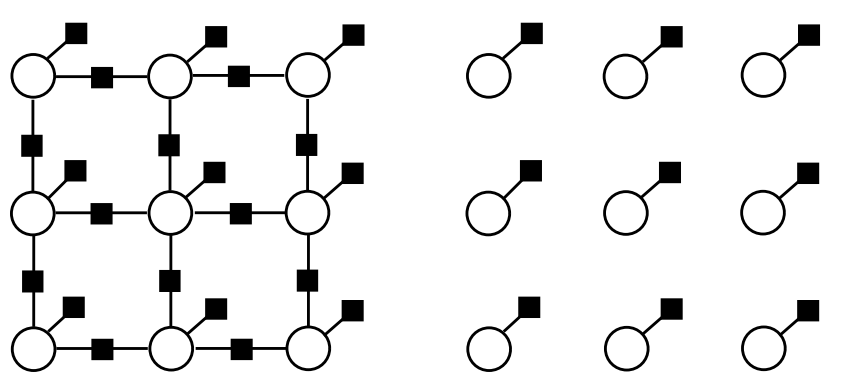
\includegraphics[scale=1]{\mlmedia/03_naive_mean_field.png}}
		\end{figure}
	\end{minipage}
\end{minipage}
~\\[.3cm]%
% % %
\subsubsection{Mean Field as Message Passing}
Now let us have a look at better mean field approximation using \emph{message passing}. %
\begin{enumerate}
	\item \itab{Initalization}
	\htab{
		Message from extremal (simplical) node factors are initialized to the factor
		\begin{equation}
		\mu_{f\rightarrow x}(x) = f(x)
		\end{equation}
		Message from extremal (simplical) variable nodes are set to unity
		\begin{equation}
		\mu_{f\rightarrow x}(x) = 1
		\end{equation}
	}
	\item \itab{Variable-to-Factor message}
	\htab{
		\begin{equation}
		\mu_{x\rightarrow f}(x) = \prod_{f_i\in\{ \NE(x)\textbackslash \{f\} \}} \mu_{f_\rightarrow x}(x)
		\label{eq:var2fac_mean_field}
		\end{equation}
	}
	\item \itab{Factor-to-Variable message}
	\htab{
		\begin{equation}
		\mu_{f\rightarrow x} \propto
			\exp\left( 
				\sum_{\mathcal{X}_f\textbackslash\{x\}} \prod_{y_i\in\{ \NE(f)\textbackslash\{x\} \}} %
				\mu_{y_i \rightarrow f}(y_i) \cdot \mu_{f \rightarrow y_i}(y_i) \cdot \log\left\{ \phi_f(\mathcal{X}_f) \right\}
				\right)
		\end{equation}
		This here is now a variational message because the messages \ensuremath{\mu_{y_i \rightarrow f}(y_i)\cdot\mu_{f \rightarrow y_i}(y_i)} guarantee that the parents \ensuremath{y_i} send their belief (i.e. the expectation of their sufficient statistics) to their children \ensuremath{y_j} while the children send their natural parameter (requires messages from the co-parents). %
	}
	\item \itab{Compute the mean field approximation}
	\htab{
		\begin{equation}
		q_i(x) \propto \prod_{f_i\in\NE(x)} \mu_{f_i \rightarrow x}(x)
		\end{equation}
	}
\end{enumerate}
\begin{minipage}[t]{1\textwidth}
	\begin{minipage}[t]{.48\textwidth}
		~\\[.75cm]
		The resulting approximation is better and still feasible because we are only looking at chains and not loopy graphs (cf. the figure to the right). %
		Nonetheless, the chain graph in the right half of the image to the right is just an example. %
		In fact arbitrary chain or tree structures are possible. %
	\end{minipage}
	\hfill
	\begin{minipage}[t]{.48\textwidth}
		\vspace*{.25cm}
		\begin{figure}[H]
		\centering\resizebox{.9\textwidth}{!}{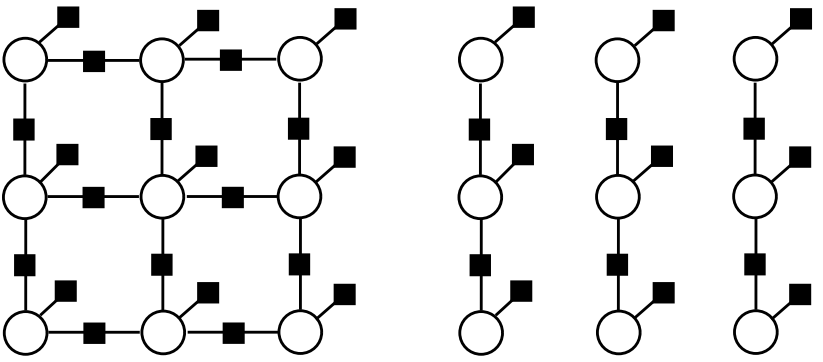
\includegraphics[scale=1]{\mlmedia/03_mean_field_message_passing.png}}
		\end{figure}
	\end{minipage}
\end{minipage}
%
%
%
\subsection{Expectation propagation}
So far, we only focused on models with discrete variables but how do we handle the continuous case? %
Generally, we need to compute an integral for the message %
\begin{equation}
\mu_{f\rightarrow x} = %
\int_{y_i\in\mathcal{X}_f\textbackslash\{x\}} \phi_f(\mathcal{X}_f) %
\prod_{y_i \in \{ \NE(f)\textbackslash\{x\} \} } \mu_{y_i \rightarrow f}(y_i) \, \mathrm{d}(\mathcal{X}_f\textbackslash\{x\})
\label{eq:factor_to_variable_msg_EP}
\end{equation}
in belief propagation. %
We can solve Equation~(\ref{eq:factor_to_variable_msg_EP}) in closed form if we assume all messages and factors to be Gaussian due to the fact that products and marginals of Gaussian are Gaussian again. %
If we cannot make this assumption, then we must assume that the messages will be a distribution in the exponential family that is %
\begin{equation*}
m(x) \propto \exp\left( \sum_j g_j(x) \cdot \nu_j \right)
\end{equation*}
with sufficient statistics \ensuremath{g_j(x)} and weights \ensuremath{\nu_j}. %
(The sufficient statistics for the Gaussian distribution are simply the first two statistical moments, i.e. \ensuremath{1,x,x^2}.) %
Now, approximate the true message \ensuremath{\mu} (which is actually a distribution) with the message \ensuremath{m} that is the closest distribution in the exponential family; thus we preserve the \emph{sufficient statistics}! %

\noindent\textbf{Note:} We use the \PROJ{~\cdot~} operator to project the messages to the exponential family at each step. %
More precisely, minimize the Kullback-Leibler divergence \KL{\mu}{m} as we did before for the mean field methods. %
We end up with belief propagation with exponential family approximations %
\begin{enumerate}
	\item \itab{Initalization}
	\htab{
		Message from extremal (simplical) node factors are initialized to the factor
		\begin{equation}
		\mu_{f\rightarrow x}(x) = f(x)
		\end{equation}
		Message from extremal (simplical) variable nodes are set to unity
		\begin{equation}
		\mu_{f\rightarrow x}(x) = 1
		\end{equation}
	}
	\item \itab{Variable-to-Factor message}
	\htab{
		\begin{equation}
		\mu_{x\rightarrow f}(x) = \prod_{f_i\in\{ \NE(x)\textbackslash \{f\} \}} \mu_{f_\rightarrow x}(x)
		\label{eq:var2fac_EP}
		\end{equation}
	}
	\item\itab{Factor-to-Variable message}
	\tab{
		\begin{equation}
		\mu_{f\rightarrow x} \propto %
		\PROJ{ %
			\mu_{x\rightarrow f}(x) \cdot %
			\int_{y_i\in\mathcal{X}_f\textbackslash\{x\}} \phi_f(\mathcal{X}_f) %
			\prod_{y_i\in\NE(f)\textbackslash\{x\}} \mu_{y_i\rightarrow f}(y_i) \, \mathrm{d}(\mathcal{X}_f\textbackslash\{x\})
		}
		(\mu_{x\rightarrow f})^{-1} %
		\end{equation}
	}
\end{enumerate}
%
%
%
\subsection{Sampling}
We learned a lot about \emph{exact inference} in the last few chapters on inference. %
However, what options do we have for problems that cannot be solved with exact inference, i.e. when the model is not tree structured? %
There are generally two approaches on how we can tackle such problems. %
\begin{enumerate}
	\item\itab{Deterministic approximation}
	\dtab{%
		- Approximate the quantity of interest\\%
		- Solve the approximation analytically\\%
		- Results depends on the quality of the approximation
	}
	\item\itab{Sampling}
	\dtab{%
		- Take the quantity of interest\\%
		- Use random samples to approximate it\\%
		- Result depends on the quality and quantity of random samples%
	}
\end{enumerate}
\emph{Sampling} allows us to get the \textit{golden standard} but we have to wait very long. %
How do we sample from \ensuremath{p(x)}, e.g. a graphical model?
We need to estimate the cumulative sum over the distribution and can select samples \ensuremath{i} with a uniform (pseudo)random number. %
\\%
\begin{minipage}[t]{1\textwidth}
	\begin{minipage}[t]{.48\textwidth}
		\subsubsection{Ancestral Sampling}%
		\fbox{\parbox[l]{1\textwidth}{%
			Assume a belief network \ensuremath{A \leftarrow B \leftarrow C} with the distribution
			\begin{equation}
			p(x) = \prod_i p(x_i\mid\PA(x_i)) = p(A\mid B) p(B\mid C) p(C).
			\end{equation}%
			We use \emph{forward sampling} to sample from the parents to the children, i.e. from the single distributions which may be difficult. %
			\textbf{Note} that each sample drawn using forward sampling is independent! %
			This is called \emph{perfect sampling} as long as the independence of the instances hold! %
			\\%
			A major problem of ancestral sampling is to have evidence, thus when we observe a subset of variables. %
			We can create a workaround if we discard all the inconsistent samples with the trade-off that this fuels inefficiency. %
		}}%
	\end{minipage}
	\hfill
	\begin{minipage}[t]{.48\textwidth}
		\subsubsection{Rejection Sampling}%
		\fbox{\parbox[l]{1\textwidth}{%
			We want to sample from \ensuremath{p(x)} but that is too difficult. %
			Assume that we can evaluate \ensuremath{p(x)} up to a constant \ensuremath{Z^{-1}}. %
			Subsequently, we evaluate the distribution as %
			\begin{equation}
			p(x) = Z^{-1} \tilde{p}(x) = Z^{-1} \prod_c \phi_c(\mathcal{X}_c)
			\end{equation}%
			and choose a \emph{proposal distribution} \ensuremath{q(x)} from which we actually can sample, more formally \ensuremath{x_i \sim q(x)}. %
			Now, we need a guarantee that the sample comes from the distribution \ensuremath{p(x)} which we actually wanted to sample from! %
			\\%
			If a uniform sample \ensuremath{u \sim U(0,1)} suffices the bound %
			\begin{equation}
				u < \frac{\tilde{p}(x_i)}{k\cdot q(x_i)}
			\end{equation}%
			for some \ensuremath{k > 1} then we will \textit{not} reject the sample \ensuremath{x_i}. %
			The efficiency of the sampler depends on \ensuremath{k}, i.e. the lower the \ensuremath{k} the more likely it gets that we accept more samples. %
			Rejection sampling is usually \emph{impractical in high dimensions} but however can be refined with adaptive techniques and multivariate sampling. %
		}}%
	\end{minipage}
\end{minipage}
~\\[.3cm]% % % % % % % % % % % % % % % % % % % % % % % %
\begin{minipage}[t]{1\textwidth}
	\begin{minipage}[t]{.48\textwidth}
		\subsubsection{Markov Chain Monte Carlo (MCMC) methods}%
		\fbox{\parbox[l]{1\textwidth}{%
			We seek to sample from a \emph{multivariate distribution} (other than in the case of rejection sampling) %
			\begin{equation}
			p(x) = Z^{-1} \tilde{p}(x)
			\end{equation}
			where the calculation of \ensuremath{Z} is intractable. %
			Here, the idea is to sample from some \ensuremath{q(x_{i+1}\mid x_i)} with a stationary distribution %
			\begin{equation}
			q_\infty(x^\prime) = \int_x q(x^\prime\mid x) q_\infty(x) \, \mathrm{d}x.
			\end{equation}%
			Given the distribution \ensuremath{p(x)}, we try to find a \emph{proposal distribution} \ensuremath{q(x^\prime\mid x)} such that \ensuremath{q_\infty(x) = p(x)} holds. %
			%Gibbs sampling can be used to obtain such a distribution for instance. %
		}}%
		~\\[.3cm] % % % % % % % % % % % % % % % % % % % % % % % % % % % % % % % % % % % % % %
		\subsubsection{Gibbs Sampling}%
		\fbox{\parbox[l]{1\textwidth}{%
			Gibbs sampling is a Markov Chain Monte Carlo method, but can also be seen as an instance of the Metropolis-Hastings. %
			The variable \ensuremath{x_i} we sample from is conditioned on its Markov blanket for sampling, thus we sample from the distribution %
			\begin{equation}
			p(x_i\mid x_{\textbackslash\{i\}}) = Z^{-1} p(x_i \mid \PA(x_i)) \prod_{j\in\CH(i)} p(x_j \mid \PA(x_j))
			\end{equation}%
			with the normalisation constant %
			\begin{equation}
			Z = \sum_{x_i} p(x_i \mid \PA(x_i)) \prod_{j\in\CH(i)} p(x_j \mid \PA(x_j)).
			\end{equation}
			The main issue with Gibbs sampling is the highly dependent states because we are sampling in terms of sequences. %
			We can overcome this issue by considering a \emph{burn-in stage} to forget our initial state but on the downside we need to sample more resulting in a longer runtime. %
			However, Gibbs sampling is one of the most widely adopted techniques for approximate inference. %
			\todo[inline]{irreducibility property, mixing coefficient}
		}}%
	\end{minipage}
	\hfill
	\begin{minipage}[t]{.48\textwidth}
		\subsubsection{Metropolis-Hastings Sampling}%
		\fbox{\parbox[l]{1\textwidth}{%
			The Metropolis-Hastings sampling is a Markov Chain Monte Carlo method. %
			Assume we are in a state \ensuremath{x_i} of the Markov chain and want to draw a new sample \ensuremath{x^\prime} from \ensuremath{p(x_i)} using a \emph{propsal distribution} \ensuremath{q(x_i)}. %
			The probability that we will use the new sample \ensuremath{x^\prime} as the next state \ensuremath{x_{i+1}} is given by %
			\begin{equation}
			\begin{aligned}
			\hat{p}(x^\prime,x_i)%
			&= \min\left( 1 , \frac{\tilde{p}(x^\prime) q(x_i|x^\prime)}{\tilde{p}(x_i) q(x^\prime|x_i)} \right)\\
			&= \min\left( 1 , \frac{p(x^\prime) q(x_i|x^\prime)}{p(x_i) q(x^\prime|x_i)} \right)%
			\end{aligned}
			\end{equation}
			where \ensuremath{\tilde{p}(x)} is an unnormalized probability density function. %
			We can show that we desire a stationary distribution \ensuremath{q_\infty(x)} of such Markov Chain as follows %
			\begin{equation}
			\begin{aligned}
			p(x) q(x^\prime|x) \hat{p}(x^\prime|x)%
			&= \min\left( p(x) q(x^\prime|x) , p(x^\prime) q(x|x^\prime) \right)\\%
			&= \min\left( p(x^\prime) q(x|x^\prime) , p(x) q(x^\prime|x) \right)\\%
			&= p(x^\prime) q(x|x^\prime) \hat{p}(x|x^\prime)
			\end{aligned}
			\end{equation}
			and if the proposal distribution is symmetric, i.e. \ensuremath{q(x_i|x^\prime) = q(x^\prime|x_i)}, we can further simplify the equation with %
			\begin{equation}
				\hat{p}(x^\prime,x_i) = \min\left( 1, \frac{p(x^\prime)}{p(x_i)} \right). %
			\end{equation}
			A common choice for the proposal ditribution is a Gaussian distribution where the mean is the current state \ensuremath{x_i} and the variance makes up the step size of the exploration. %
			In this particular case, a large variance results in many rejections and a small variance results in a slow exploration. %
		}}%
		~\\[.3cm] % % % % % % % % % % % % % % % % % % % % % % % % % % % % % % % % % % % % % % % % % % %
		\subsubsection{Block Gibbs Sampling}%
		\fbox{\parbox[l]{1\textwidth}{%
			Instead of sampling from \ensuremath{p(x)}, we sample from \ensuremath{p(x,u)} such that %
			\begin{equation}
			p(x) = \int p(x,u) \, \mathrm{d}u \qquad\text{ or }\qquad p(x) = \sum_u p(x,u).
			\end{equation}
			To sample from the joint distribution \ensuremath{p(x,u)}, we iterate between sampling \ensuremath{p(u|x)} and sampling \ensuremath{p(x|u)}. %
			This is an useful sampling algorithm for certain MRFs and RBMs (Restricted Boltzmann Machines) where \ensuremath{p(u|x)} makes sampling easy and \ensuremath{p(x|u)} is Gaussian so makes it easy to sample as well. %
		}}%
	\end{minipage}
\end{minipage}
%~\\[.3cm]% % % % % % % % % % % % % % % % % % % % % % % %
%\begin{minipage}[t]{1\textwidth}
%	\begin{minipage}[t]{.48\textwidth}
%		% Gibbs sampling
%	\end{minipage}
%	\hfill
%	\begin{minipage}[t]{.48\textwidth}
%		% Gibbs block sampling
%	\end{minipage}
%\end{minipage}
~\\%[.3cm]% % % % % % % % % % % % % % % % % % % % % % % %
\begin{minipage}[t]{1\textwidth}
	\begin{minipage}[t]{.48\textwidth}
		\subsubsection{Slice Sampling}%
		\fbox{\parbox[l]{1\textwidth}{%
			A disadvantage of the Metropolis-Hastings algorithm is the dependence of finding a good proposal distribution that involves setting step-size parameters of such a distribution to appropriate values. %
			Slice sampling tries to overcome this issue by directly sampling uniformly under the curve of an unnormalized probability density function \ensuremath{\tilde{p}(x) \propto p(x)} of the probability density function \ensuremath{p(x)}, i.e. drawing samples \ensuremath{(x^\prime,u^\prime)\sim p(x,u)}. %
			We sample from the joint distribution %
			\begin{equation}
			p(x,u) = \begin{cases} Z_{\tilde{p}(x)}^{-1}, & \text{if } 0 \leq u \leq \tilde{p}(x)\\ 0, & \text{otherwise.} \end{cases}
			\end{equation}
			with normalization constant \ensuremath{Z_{\tilde{p}(x)}^{-1}} corresponding to \ensuremath{\tilde{p}(x)}. %
			After a sample from the above distribution has been drawn, we can obtain a sample from the marginal distribution \ensuremath{p(x)} by dropping the value \ensuremath{u}. %
			We show that this holds as follows %
			\begin{equation}
			\int p(x,u) \, \mathrm{d}u = 0 + \int_{0}^{\tilde{p}(x)} Z_{\tilde{p}(x)}^{-1} \,\mathrm{d}u + 0 = Z_{\tilde{p}(x)}^{-1} \tilde{p}(x) = p(x).
			\end{equation}
			Let us take a step back and focus on how to sample from the joint distribution \ensuremath{p(x,u)}. %
			We use \emph{Gibbs sampling} and alternating draw samples from distributions as follows%
			\begin{align*}
			u &\sim p(u|x) = U(0,\tilde{p}(x))\\
			x &\sim p(x|u) = \begin{cases} 1, & \text{if } \tilde{p}(x) \geq u\\ 0, & \text{otherwise.} \end{cases}
			\end{align*}
			Here the sample set \ensuremath{\left\{ x \; : \; u \leq \tilde{p}(x) \right\}} defines a \textit{slice} and hence the name of the sampling algorithm. %
			\fixcfigure{.9}{\mlmedia/03_slice_sampling.png}%
			\captionof{figure}{Slice sampling from the area underneath the curve and dropping \ensuremath{u}.}
		}}%
	\end{minipage}
	\hfill
	\begin{minipage}[t]{.48\textwidth}
		\subsubsection{Hybrid / Hamiltonian Monte Carlo}%
		\fbox{\parbox[l]{1\textwidth}{%
			Metropolis-Hastings sampling explores the proposal distribution with random walk. %
			This approach is not very efficient for the exploration of strongly correlated distributions. %
			We aim to take the model distribution \ensuremath{p(x)} into account for proposal distributions. %
			We start with considering the energy corresponding to the distribution %
			\begin{equation}
			p(x) \propto \exp\left\{ -E(x) \right\}
			\end{equation}%
			with the energy term %
			\begin{equation}
				E(x) = -\log\left\{ \tilde{p}(x) \right\}.
			\end{equation}
			The energy \ensuremath{E(x)} describes the potential energy of a physical system. %
			We aim to describe the \emph{total energy} (\emph{Hamiltonian}) %
			\begin{equation}
			H(x,v) = E(x) + K(\vec{v})
			\end{equation}
			where \ensuremath{K(\vec{v}) = (2)^{-1} \vec{v}^\top \mat{M}^{-1} \vec{v}} is the kinetic energy parameterized by the velocity. %
			Furthermore, we assume unit mass, i.e. \ensuremath{\mat{M} = \mat{I}}, of the kinetic energy. %
			A particle that moves through the system (e.g. transition in the Markov chain) preserves the total energy \ensuremath{H(\vec{x},\vec{v}) = H(\vec{x}^\prime,\vec{v}^\prime)} and if we reverse the velocity \ensuremath{\vec{v}^\prime}, the particle will return from \ensuremath{\vec{x}^\prime} to \ensuremath{\vec{x}} with velocity \ensuremath{-\vec{v}} at arrival. %
			The essential idea is to define a joint distribution %
			\begin{equation}
			p(\vec{x},\vec{v}) \propto \exp\left\{ -E(\vec{x}) -K(\vec{v}) \right\}
			\end{equation}
			following the Hamiltonian energy with Gaussian distributed velocity \vec{v} that is independent of position \vec{x}. %
			To transition in our system, we do the following: %
			\begin{enumerate}
				\item Sample the velocity \begin{equation} \vec{v} \sim p(\vec{v}) \propto \exp\left\{ -K(\vec{v}) \right\} \end{equation}
				\item Simulate Hamiltonian dynamics for some time interval arriving at \ensuremath{(\vec{x}^\prime,\vec{v}^\prime)} with the property \begin{equation} q(\vec{x}^\prime, \vec{v}^\prime | \vec{x}, \vec{v}) = q(\vec{x}, \vec{v} | \vec{x}^\prime, \vec{v}^\prime) \end{equation}
				\item Accept the move to \ensuremath{(\vec{x}^\prime,\vec{v}^\prime)} with maximal probability because following holds \begin{equation} p(\vec{x}^\prime, \vec{v}^\prime) = p(\vec{x}, \vec{v}) \end{equation}
			\end{enumerate}
			However, we cannot simulate Hamiltonian dynamics exactly but we can use \emph{numerical methods to solve the differential equations} (for step 2), i.e. the leapfrog method, and \emph{Metropolis-Hastings} sampling to accept or reject the transition to the new state (step 3). %
		}}%
	\end{minipage}
\end{minipage}
%
%
%
% % % % % % % % % % % % % % % % % % % % %
\section{Learning in graphical models}
The focus shifts from inference in graphical models to learning parameters of graphical models. %
In the last chapter, we presented many algorithms to infer model distributions directly and approximately. %
Now we need to tweak the (hyper)parameters of such model distributions. %
We will now learn about algorithms to do so for the different model distributions. %
%
%
%
\subsection{Learning in belief networks}
A belief network will be specificed by a model distribution \ensuremath{p(x)} after inference. %
However, we need to estimate optimal parameters \ensuremath{\theta} to shape our model distribution to our needs. %
This change in shape can be understand in terms of plasticity and we tend to call this issue \emph{learning}. %
For the basic setup, we are given the parameterized model distribution %
\begin{equation}
p(x\mid\theta)
\end{equation}
and training data \ensuremath{\mathcal{D}} corresponding to the distribution or our problem task. %
Basically, there are two different approaches on how to obtain the most optimal parameters \ensuremath{\theta^*} %
\begin{enumerate}
	\item Point estimators (finding exactly one \ensuremath{\theta^*}) and
	\item Bayesian learning (integrating out all \ensuremath{\theta}). %
\end{enumerate}
%
%
%
\begin{topic}{.3cm}{Point estimator: Maximum Likelihood for Belief Networks}
	The most common point estimator technique is the maximum likelihood estimate approach. %
	Recall that maximizing the maximum likelihood of Equation~(\ref{eq:bayesian_network}) corresponds to \emph{minimizing the Kullback-Leibler divergence} of the empirical distribution \ensuremath{q(x)} (from our data) and our model distsribution \ensuremath{p(x)}. %
	\begin{equation}
	\begin{aligned}
	\underset{p}{\arg\min}\left\{ \KL{q}{p} \right\} %
	&= \underset{p}{\arg\min}\left\{  -\E[q(x)]{ \sum_{i=1}^{K} \log\left\{ p(x_i\mid\PA(x_i)) \right\} } + \text{const}  \right\}\\ %
	&= \underset{p}{\arg\min}\left\{  -\sum_{i=1}^{K} \E[q(x_i\mid\PA(x_i))]{ \log\left\{ p(x_i\mid\PA(x_i)) \right\} } + \text{const}  \right\}\\ %
	&= \underset{p}{\arg\min}\left\{  \sum_{i=1}^{K} \left[  \E[q(x_i\mid\PA(x_i))]{ \log\left\{ p(x_i\mid\PA(x_i)) \right\} } - \E[q(x_i\mid\PA(x_i))]{ \log\left\{ q(x_i\mid\PA(x_i)) \right\} }  \right]  \right\}\\ %
	&= \underset{p}{\arg\min}\left\{  \sum_{i=1}^{K} \KL{q(x_i\mid\PA(x_i))}{p(x_i\mid\PA(x_i))}  \right\}\\ %
	\end{aligned}
	\end{equation}
\end{topic}
% % %
\newpage
\begin{topic}{.3cm}{Bayesian Learning of Belief Networks}
	The maximum likelihoood estimate approach is a heuristic. %
	To use bayesian learning we need to define a \emph{prior on the parameters} and then \emph{compute the posterior} %
	\begin{equation}
		p(\theta\mid\mathcal{D}) \propto p(\mathcal{D}\mid\theta) p(\theta)
	\end{equation}
	Here we need to learn a parameter for each factor because each factor corresponds to a probability distribution and the \emph{prior distribution decomposes} (and hence also the posterior distribution decomposes) into different parts due to independence. %
	For binary events, we shall assume the Binomial distribution for the likelihood but how do we model the prior distribution? %
	We shall choose a beta distribution %
	\begin{equation}
	p(\theta) %
	= B\left( \theta \middle| \alpha, \beta \right) %
	= \frac{\Gamma(\alpha)\cdot\Gamma(\beta)}{\Gamma(\alpha+\beta)} \theta^{\alpha-1} \cdot (1-\theta)^{\beta-1}
	\end{equation}
	with the Gamma function %
	\begin{equation}
	\Gamma(n) = \int_0^\infty t^{n-1} \exp\left\{-t\right\} \, \mathrm{d}t = (n+1)!
	\end{equation}
	for the prior because it represents our belief for binary events and is also a conjugate prior. %
	If we choose now to model multiple binary events, as it is the case for a whole bayesian network, we can model our prior with a \emph{Dirichlet distribution} and the likelihood with a \emph{Multinomial distribution} which is both the multivariate equivalent of the Beta distribution and the Binomial distribution, respectively. %
\end{topic}
%
%
%
\subsection{Learning in Markov networks}
A Markov Network is defined on (not necessarily maximal) cliques that is %
\begin{equation}
p(x|\theta) = Z(\theta)^{-1} \prod_c \phi_c(x_c|\theta_c)
\label{eq:Markov_network_likelihood}
\end{equation}
with clique variables \ensuremath{x_c} and partition function %
\begin{equation}
Z(\theta) = \int \prod_c \phi_c (x_c|\theta_c) \, \mathrm{d}x.
\end{equation}%
Now we are given training data \ensuremath{\mathcal{D}} again to do either maximum likelihood or Bayesian learning. %
For \emph{belief networks}, the posterior decomposed into different parts due to the independence of prior but this is not the case for Markov Networks in general. %
The main difficulty is to estimate the unknown partition function \ensuremath{Z(\theta)}. %
\newpage
\begin{topic}{.3cm}{Point estimator: Maximum Likelihood for Markov networks}
	The most common point estimator technique is the maximum likelihood estimate approach and hence we will use the log variant of it here (for numerical stability). %
	The likelihood of a Markov network is defined in Equation~(\ref{eq:Markov_network_likelihood}) and the log variant derives as follows %
	\begin{equation}
	\begin{aligned}
	\log\{p(x\mid\theta)\}
	&= \sum_n \sum_c \log\left\{ \phi_c(x_c^n) \middle| \theta_c \right\} - \sum_n \log\left\{ Z(\theta) \right\} \\
	&= N\cdot N^{-1} \sum_n \sum_c \log\left\{ \phi_c(x_c^n) \middle| \theta_c \right\} -  N\cdot \log\left\{ Z(\theta) \right\} \\
	&= N\cdot \E[q(x;\mathcal{D})]{\sum_c \log\left\{ \phi_c(x_c) \middle| \theta_c \right\}} -  N\cdot \log\left\{ Z(\theta) \right\} \\
	\end{aligned}
	\end{equation}
	where \ensuremath{q(x;\mathcal{D}) = N^{-1} \sum_n \delta(x-x^n)} is the empirical distribution. %
	To obtain the optimal parameter \ensuremath{\theta^*}, we need to take the derivative of the log-likelihood with respect to \ensuremath{\theta} (and setting it to zero) and we obtain %
	\begin{equation}
	\begin{aligned}
	\frac{\partial}{\partial\theta_d} \log\{p(x\mid\theta)\}
	&= \frac{\partial}{\partial\theta_d} \left[  N\cdot \E[q(x;\mathcal{D})]{\sum_c \log\left\{ \phi_c(x_c) \middle| \theta_c \right\}} -  N\cdot \log\left\{ Z(\theta) \right\}  \right] \\
	&= N\cdot \E[q(x;\mathcal{D})]{\sum_c \frac{\partial}{\partial\theta_d} \log\left\{ \phi_c(x_c) \middle| \theta_c \right\}} -  N\cdot \frac{\partial}{\partial\theta_d} \log\left\{ Z(\theta) \right\} \\
	&= N\cdot \E[q(x;\mathcal{D})]{\frac{\partial}{\partial\theta_d} \log\left\{ \phi_d(x_d) \middle| \theta_d \right\}} -  N\cdot \frac{\partial}{\partial\theta_d} \log\left\{ \int \prod_c \phi_c\left(x_c \middle| \theta_c \right) \,\mathrm{d}x \right\} \\
	&= N\cdot \E[q(x;\mathcal{D})]{\frac{\partial}{\partial\theta_d} \log\left\{ \phi_d(x_d) \middle| \theta_d \right\}} %
		- N\cdot Z(\theta)^{-1} \cdot \frac{\partial}{\partial\theta_d} \int \prod_c \phi_c\left(x_c \middle| \theta_c \right) \,\mathrm{d}x \\
	&= N\cdot \E[q(x;\mathcal{D})]{\frac{\partial}{\partial\theta_d} \log\left\{ \phi_d(x_d) \middle| \theta_d \right\}} %
		- N\cdot Z(\theta)^{-1} \cdot \int \prod_c \frac{\partial}{\partial\theta_d} \phi_c\left(x_c \middle| \theta_c \right) \,\mathrm{d}x \\
	&= N\cdot \E[q(x;\mathcal{D})]{\frac{\partial}{\partial\theta_d} \log\left\{ \phi_d(x_d) \middle| \theta_d \right\}} %
		- N\cdot Z(\theta)^{-1} \cdot \int \frac{\partial}{\partial\theta_d} \phi_d\left(x_d \middle| \theta_d \right) \cdot \prod_{c\neq d} \phi_c\left(x_c \middle| \theta_c \right) \,\mathrm{d}x \\
	&= N\cdot \E[q(x;\mathcal{D})]{\frac{\partial}{\partial\theta_d} \log\left\{ \phi_d(x_d) \middle| \theta_d \right\}} %
		- N\cdot Z(\theta)^{-1} \cdot \int \frac{\partial}{\partial\theta_d} \log\left\{\phi_d\left(x_d \middle| \theta_d \right)\right\} \cdot \prod_{c} \phi_c\left(x_c \middle| \theta_c \right) \,\mathrm{d}x \\
	&= N\cdot \E[q(x;\mathcal{D})]{\frac{\partial}{\partial\theta_d} \log\left\{ \phi_d(x_d) \middle| \theta_d \right\}} %
		- N\cdot \E[p(x|\theta)]{ \frac{\partial}{\partial\theta_d} \log\left\{\phi_d\left(x_d \middle| \theta_d \right)\right\} }.
	\end{aligned}
	\end{equation}%
	However, this requires inference because we need to take an average over the model distribution \ensuremath{p(x|\theta)}. %
	We can extend this even further with an \emph{energy view} of Markov Random Fields. %
\end{topic}
%
\newpage
\begin{topic}{.3cm}{Energy of Markov Networks}
	We can use energy to express correlation in a system. %
	Therefore, we describe a Markov Network by a \emph{Gibbs distribution} / \emph{Boltzmann distribution} %
	\begin{equation}
	p(x\mid\theta) = Z(\theta,T)^{-1} \exp\left\{ -T^{-1} E(x;\theta) \right\}
	\label{eq:gibbs_distribution}
	\end{equation}%
	with temperature \ensuremath{T} and the \emph{potentials} defined as %
	\begin{equation}
	E(x;\theta) = \sum_c E_c(x_c;\theta_c). %
	\end{equation}
	The partition function is given by the sum over all \ensuremath{x} of Equation~(\ref{eq:gibbs_distribution}). %
	We write the log likelihood gradient as %
	\begin{equation}
	\frac{\partial}{\partial\theta_d} p(x\mid\theta) = -N \cdot \E[q(x;\mathcal{D})]{\frac{\partial}{\partial\theta_d}E(x;\theta)} + N \cdot \E[p(x\mid\theta)]{\frac{\partial}{\partial\theta_d}E(x;\theta)}
	\end{equation}
	There is a \emph{closed form solution} available for maximum (log) likelihood in \emph{decomposable Markov networks}. %
	The type of solution can be characterized by unconstrained potentials and exponential family models. %
	Hence, we cannot obtain a closed form solution for non-decomposable Markov networks with constrained forms of the potential and are limited to \emph{approximate inference with sampling} or approximate the parameter with moment matching methods. %
\end{topic}
% % % % % % % % % %
\begin{topic}{.3cm}{Unconstrained potentials}
	Unconstrained potentials are important to obtain a closed form maximum likelihood solution for Markov networks. %
	If there are no constraints on the potentials, i.e. we can obtain the gradient of real distribution average and do gradient descent. %
	Otherwise, if we have constraints on the potentials, we need to go for constraint optimization techniques. %
\end{topic}
% % % % % % % % % %
\newpage
\begin{topic}{.3cm}{Decomposable Markov Networks}
	A Markov network si called \emph{decomposable} when we can write %
	\begin{equation}
		p(x_1, \ldots, x_n) = \frac{\prod_c p(x_c)}{\prod_s p(x_s)}
	\end{equation}
	where \ensuremath{p(x_c)} is a \emph{maximal clique} and \ensuremath{p(x_s)} is called a \emph{seperator}. %
	An example for a decomposable Markov network with its Clique Graph (at the right; also called \emph{junction tree}) and the decomposable Markov network is shown in the following figure. %
	\fixcfigure{.55}{\mlmedia/03_decomp_MN.png}
	The clique graph of the Markov network in the left is given by %
	\begin{equation}
		p(a,b,c,d) = Z^{-1} \phi(a,b,c) \phi(b,c,d)
	\end{equation}
	where we can write the marginals over \ensuremath{a} and \ensuremath{d} as %
	\begin{align*}
		p(b,c,d) \cdot Z &= \phi(b,c,d) \sum_a \phi(a,b,c)\\
		p(a,b,c) \cdot Z &= \phi(a,b,c) \sum_d \phi(b,c,d)
	\end{align*}
	respectively to conclude that the product of the two marginals %
	\begin{align*}
		Z^2 \cdot p(a,b,c) p(b,c,d)
		&= \left( \phi(b,c,d) \sum_a \phi(a,b,c) \right) \cdot \left( \phi(a,b,c) \sum_d \phi(b,c,d) \right) \\
		&= Z^2 \cdot p(a,b,c,d) \sum_{a,d} p(a,b,c,d)
	\end{align*}%
	leads to the representation of the Markov network (in the right half of the above figure) as follows %
	\begin{equation}
		p(a,b,c,d) = \frac{p(a,b,c) p(b,c,d)}{p(b,c)}. %
	\end{equation}
	The \emph{most important insight} here is that we can rewrite the distribution of a Markov network in terms of its marginals on the variables in the original cliques. %
	The structure remains the same and all that has changed is that the original clique potentials have been replaced by the marginals of the distribution and the seperator by the marginal defined on the seperator variables. %
\end{topic}
%
%
%
\subsection{Conditional Random Fields}
A \emph{Conditional Random Field} is defined as a conditional distribution %
\begin{equation}
	p\left( \vec{y} \middle| \vec{x} \right) = {Z(\vec{x}, \theta)}^{-1} \exp\left\{ -E(\vec{x},\vec{y},\theta) \right\}
\end{equation}
where the partition function now depends on the input vector %
\begin{equation}
	Z(\vec{x},\theta) = \sum_{\vec{y}\in\mathcal{Y}} \exp\left\{ -E(\vec{x},\vec{y},\theta) \right\}. %
\end{equation}
A Conditional Random Field is similar to a Markov Random Field (special case of the Markov Network), but the condition on the input \ensuremath{\vec{x}} makes a huge difference for the partition function! %
However, the potentials are - as in the Markov Random Fields - implicitly modeled in the energy term. %
The difference between the Conditional Random and Markov Random Fields is that the \emph{Conditional Random Fields describe a discriminant approach} while the Markov Random Fields describe a generative approach. %
The first advantage of learning \ensuremath{p(\vec{y}|\vec{x})} instead of \ensuremath{p(\vec{x},\vec{y})} is that the learning process is easier in general and only depends on the \ensuremath{\vec{y}}'s and the second advantage is that we do not need very high-dimensional potentials. %
However, the discriminative approach is tied to the predicition problem \ensuremath{p(\vec{y}|\vec{x})}. %
\begin{topic}{0.3cm}{Maximum likelihood for Conditional Random Fields}
	The maximum likelihood for Conditional Random Fields (or \emph{conditional likelihood}) is given by %
	\begin{equation}
	\begin{aligned}
		p(\theta;\vec{x},\vec{y})
		&= \sum_n \log\left\{ p( \vec{y}_n | \vec{x}_n , \theta ) \right\}\\
		&= -\sum_n E( \vec{y}_n ,\vec{x}_n , \theta ) - \log\left\{ Z(\vec{x}_n,\theta) \right\}
	\end{aligned}
	\end{equation}
	where, again, knowing the partition function \ensuremath{Z} makes learning tractable in tree-like structures. %
	One ususally uses exponential family Conditional Random Fields that are of the form %
	\begin{equation}
		p(\vec{y}|\vec{x},\theta) = Z(\vec{x},\theta)^{-1} \exp\left\{ \theta^\top \phi(\vec{x},\vec{y}) \right\}
	\end{equation}
	with \ensuremath{\phi(\vec{x},\vec{y})} being some fixed feature functions. %
	The maximum likelihood problem then becomes %
	\begin{equation}
		\theta^* = \underset{\theta\in\mathbb{R}^D}{\arg\max}\left\{ \sum_n \theta^\top \phi(\vec{x}_n,\vec{y}_n) - \sum_n \log\left\{ Z(\vec{x}_n,\theta)^{-1} \right\}  \right\}
		\label{eq:CRF_ML}
	\end{equation}
	and with this choice, the problem becomes linear in the parameters \ensuremath{\theta} and hence convex. %
\end{topic}
% % % % % % % % % % % % % %
\begin{topic}{0.3cm}{Regularized Maximum Conditional Likelihood}
	Instead of solving Equation~(\ref{eq:CRF_ML}), we can solve the \emph{regularized maximum conditional likelihood}
	\begin{equation}
	\begin{aligned}
		\theta^*
		&= \underset{\theta\in\mathbb{R}^D}{\arg\max} \left\{ p(\theta) \prod_{n=1}^N p(\vec{y}_n | \vec{x}_n , \theta ) \right\}\\
		&= \underset{\theta\in\mathbb{R}^D}{\arg\min} \left\{ -\log\left\{ p(\theta) \right\} -\sum_{n=1}^N \theta^\top \phi(\vec{x}_n,\vec{y}_n) + \sum_n \log\left\{ Z(\vec{x}_n,\theta) \right\} \right\}
	\end{aligned}
	\end{equation}
	which is more robust to overfitting due to the introduced prior. %
	For a Gaussian prior, we obtain the following solution %
	\begin{equation}
		\theta^* = \underset{\theta\in\mathbb{R}^D}{\arg\min}\left\{ \lambda ||\theta||^2 - \sum_{n=1}^N \theta^\top \phi(\vec{x}_n,\vec{y}_n) + \sum_n \log\left\{ Z(\vec{x}_n,\theta) \right\} \right\}. %
	\end{equation}
\end{topic}
% % % % % % % % % % % % % % %
\newpage
\begin{topic}{0.3cm}{Ising / Potts model}
	The Ising / Potts model can be used for \emph{image denoising applications}. %
	Here, we assume a \emph{Markov Random Field} with observed noisy pixels \ensuremath{x_i \in \{-1,+1\}} and true underlying image pixel \ensuremath{y_i \in \{-1,+1\}}. %
	We \textit{restrict} ourselves to three parameters \ensuremath{h,\beta,\eta}, i.e. the energy function is of the form %
	\begin{equation}
		E(\vec{x},\vec{y}) = h \sum_i \vec{y}_i - \beta \sum_{i\sim j} \vec{y}_i \vec{y}_j - \eta \sum_i \vec{x}_i \vec{y}_i
	\end{equation}
	and the complete \emph{Ising model} has the form %
	\begin{equation}
		p(\vec{x},\vec{y}) = Z^{-1} \exp\left\{ -E(\vec{x},\vec{y}) \right\}. %
	\end{equation}
	However, we implicitly model \ensuremath{p(\vec{y}|\vec{x})} because we have no knowledge about the true underlying image \ensuremath{\vec{y}}. %
	And hence we seek the solution given by %
	\begin{equation}
		\vec{y}^* = \underset{\vec{y}}{\arg\max} \left\{ p(\vec{y}|\vec{x}) \right\}. %
	\end{equation}
	We cannot obtain the soltuion directly, i.e. in closed form. %
	So, how do we infer the distribution then? %
\end{topic}
% % % % % % % % % % % % % % %
\begin{topic}{0.3cm}{Iterated Conditional Means (ICM)}
	We can obtain an approximated solution with the \emph{Iterated Conditional Means} method. %
	Given the noisy image \ensuremath{\vec{x}}, we simply initialize our true underlying image with the noisy image \ensuremath{\vec{y} = \vec{x}}. %
	Now it is crucial to pick solely one pixel after another in random or fixed order and minimize the energy for this specific pixel for all possible pixel values (here: \ensuremath{\vec{y}_i\in\{1,+1\}}). %
	Iterate with this procedure until convergence (choose an appropriate convergence criterium). %
	
	\noindent\textbf{Note:} Iterated Conditional Means will only find a \emph{local maximum solution}. %
	In general we can do better with minimizing the (true) posterior expected loss %
	\begin{equation}
		\vec{y}^* = \underset{\vec{y}^\prime}{\arg\min}\left\{ \int_{\vec{y}} L(\vec{y}^\prime,\vec{y}) p(\vec{y}|\vec{x}) \right\}
	\end{equation}
	where we still need to be careful with the choice of the loss function \ensuremath{L}! %
	However, this approach will likely only succeed in finding better local maxima for the 0/1 loss which must be sufficiently appropriate for the given application!
\end{topic}
%
%
%
\subsection{Latent Variable Models}
In Latent Variable Models, there are unobserved variables during the training for which we seek a solution. %
There are two possible solutions presented here to solve for \emph{Latent Variable Models}. %
The first solution would be to margnialize out the unobserved variables which may lead to complex dependencies (and other problems). %
The other approach would include the following algorithms. %
\newpage
% % % % % % % % % % % % % % %
\begin{topic}{0.3cm}{Gaussian Mixture Models (GMM) / Mixture of Gaussians (MoG)}
	The idea of Gaussian Mixture Models is to either estimate a probability density or cluster data where %
	\begin{equation}
		p(\vec{x}|\theta) = \sum_{j=1}^m p(\vec{x}|\theta_j) p(j)
	\end{equation}
	is a smooth density approximation with \ensuremath{m} many Gaussians. %
	We identify the different terms formally as %
	\begin{align}
		p(\vec{x}|\theta) &= \sum_{j=1}^m {\color{Red}p(\vec{x}|\theta_j)} {\color{Orange}p(j)} \\
		{\color{Red} p(\vec{x}|\theta_j)} &= \mathcal{N}(\vec{x}|\mu_j,\sigma^2_j) \\
		{\color{Orange} p(j)} &= \pi_j \text{ with } 0\leq\pi_j \leq 1, ~\sum_{j=1}^m \pi_j = 1
	\end{align}
	Hence there are \ensuremath{3\cdot m} parameters to learn and the mixture density is a probability distribution! %
	
	\begin{minipage}[t]{1\textwidth}
		\begin{minipage}[t]{.58\textwidth}
			We can view the Gaussian Mixture Model as a particular Bayesian network (see the figure to the right). %
			But how do we sample from such a mixture model? %
			Basically, we want to sample from \ensuremath{ p(\vec{x}|\theta) = \sum_j \pi_j p(\vec{x}|\theta_j) } and hence we first draw a \ensuremath{ j\sim p(j) } and then draw a \ensuremath{ x\sim p(\vec{x}|\theta_j) }. %
			This is \emph{Ancestral sampling} and we can use it for approximate inference of the latent distribution. %
			The maximum likelihood solution then yields for the paarameters %
			\begin{align}
				\vec{\pi}_j &= {n_j}^{-1} \cdot n \\
				\vec{\mu}_j &= {n_j}^{-1} \sum_{i:l_i = j} \vec{x}_i \\
				\mat{\Sigma}_j &= {n_j}^{-1} \sum_{i:l_i=j} (\vec{x}_i - \vec{\mu}_i) (\vec{x}_i - \vec{\mu}_i)^\top
			\end{align}
			with labels \ensuremath{l_i} of sample \ensuremath{\vec{x}_i}, \ensuremath{n} as the total number of labels and \ensuremath{n_j} as the number of samples with label \ensuremath{j}. %
		\end{minipage}
		\hfill
		\begin{minipage}[t]{.38\textwidth}
			\fixcfigure[!]{0.45}{\mlmedia/03_GMM.png}
		\end{minipage}
	\end{minipage}
	But here we do not know anything about the class label assignments. %
	We can \textit{simply} guess them, based on the current estimated mixture distribution, as %
	\begin{equation}
		\hat{p}(j|i) = p(l_i = j| \vec{x}_i,\theta), \qquad \sum_{j=1}^m \hat{p}(i|j) = 1, \quad \forall i = 1,\ldots, n
	\end{equation}
	with %
	\begin{equation}
	p(l_i = j| \vec{x}_i,\theta)
	= \frac{p(l_i = j,\vec{x}|\theta)}{p(\vec{x}|\theta)}
	= \frac{p(\vec{x}|\theta_j) p(l_i = j)}{\sum_{j=1}^m p(\vec{x}|\theta_j)p(j)}. %
	\end{equation}
	Given this soft assignment estimates, we can formulate the \emph{Expectation Maximization} (\emph{EM}) algorithm for this issue where in the \emph{E-step} we softly assign samples to mixture components %
	\begin{equation}
		\hat{p}(j|i) \leftarrow p(l_i=j|\vec{x}_i,\theta) \qquad \forall j = 1,\ldots,m \quad \forall i = 1,\ldots,n
	\end{equation}
	and in the \emph{M-step} we re-estimate parameters based on the soft assignments %
	\begin{align}
		\hat{n}_j &\leftarrow \sum_{i=1}^n \hat{p}(j|i) & \vec{\hat{\pi}}_j &\leftarrow \frac{\hat{n}_j}{n} \\
		\vec{\hat{\mu}}_j &\leftarrow \frac{1}{\hat{n}_j} \sum_{i=1}^n \hat{p}(j|i) \vec{x}_i & \mat{\hat{\Sigma}} &\leftarrow \frac{1}{\hat{n}_j} \sum_{i=1}^n \hat{p}(j|i) (\vec{x}_i - \vec{\hat{\mu}}_j) (\vec{x}_i - \vec{\hat{\mu}}_j)^\top.
	\end{align}
\end{topic}
% % % % % % % % % % % % % % %
Next, we are going to introduce the \emph{Latent Semantic Analysis} for which we need to define some more terminology. %
We define the \emph{term frequency} (\emph{TF}) of one document \ensuremath{d} as %
\begin{equation}
	\mathrm{tf}(d,w) = \frac{n(d,w)}{\sum_k n(d,k)}
\end{equation}
with \ensuremath{n(d,w)} as the number of occurences of word \ensuremath{w} in document \ensuremath{d}. %
Furthermore, the \emph{inverse document frequency} (\emph{IDF}) of a corpus %
\begin{equation}
	\mathrm{idf}(w) = \log\left\{ \frac{n}{|\{ d| n(d,w) \neq 0 \}|} \right\}
\end{equation}
can be used to obtain a weighting of entries according to importance %
\begin{equation}
	\mathrm{\text{tf-idf}}(d,w) = \mathrm{tf}(d,w) \cdot \mathrm{idf}(d).
\end{equation}
Often, the document-term matrices are huge, e.g. the internet. %
The challenges we encounter are the following. %
\begin{itemize}
	\item \emph{Compactness}: few search terms with rare redundancy
	\item \emph{Variability}: synonyms and semantically related terms, expression, writing styles, etc.
	\item \emph{Ambiguity}: Terms with multiple senses (polysems)
	\item \emph{Quality \& Authority}: Correlation between quality and relevance
\end{itemize}
\begin{topic}{0.3cm}{Latent Semantic Analysis (LSA)}
	Assume we are given a matrix \ensuremath{\mat{A}} that encodes the data in some way, e.g. co-occurence counts. %
	This matrix will be in general too large, or too complicated, or may have missing or noisy entries, or lack structure. %
	So we try to explore a latent structure underlying the data to explain the entries. %
	We expect to obtain a structure that e.g. encodes semantic topics. %
	The common approach to reveal such a structure is to approximately factorize the matrix, i.e. %
	\begin{equation}
		\mat{A} \approx \underbrace{\tilde{\mat{A}}}_{\text{approximation}} = \underbrace{\mat{L}}_{\text{left factor }} \underbrace{\mat{R}}_{\text{ right factor}}. %
	\end{equation}
	We can obtain such a factorization with the singular value decomposition %
	\begin{equation}
		\mathrm{SVD}(\mat{A}) = \underbrace{\mat{L}}_{\text{left singular eigenvectors }} \underbrace{\mat{\Sigma}}_{\text{ singular values }} \underbrace{\mat{R}}_{\text{ right singular eigenvectors}}. %
	\end{equation}
	Here, \ensuremath{\mat{\Sigma}} is a diagonal matrix where we set the smallest singularvalues (the ones which are close to zero) to zero, such that we can solve our approximation problem %
	\begin{equation}
		\mat{A}^* = \underset{ \hat{\mat{A}}:rank(\hat{\mat{A}}) = q }{ \arg\min } \left\{ || \mat{A} - \hat{\mat{A}} || \right\}
	\end{equation}
\end{topic}
We can do even better than with Latent Semantic Analysis by reformulating the Latent Semantic Analysis with probabilities. %
For the \emph{probabilistic Latent Semantic Analysis} (\emph{pLSA}), we try to maximize the quantity %
\begin{equation}
	p(R_d = 1|r) \propto p(r|R_d = 1) p(R_d=1)
\end{equation}
where \ensuremath{R_d} is the document relevance and \ensuremath{r} is a query or set of words. %
We cannot obtain a solution directly but we can use the \emph{Expectation Maximization} (\emph{EM}) algorithm to maximize the likelihood. %
%
%
%